%!TEX root = CooperBarba2014.tex

The implicit-solvent model describes a molecular system as a set of continuum dielectric regions, and computes the mean-field potential using electrostatics. 
For the case where a protein is dissolved in a solvent, we require two of such regions: inside and outside the protein, interfaced by the solvent-excluded surface (\ses). 
The \ses determines the closest a water molecule can get to the protein, and we generate it by rolling a spherical probe of the size of a water molecule around the protein. 
The dielectric constant inside the protein is low ($\epsilon= 2\text{ to }4$) and there are point charges to mimic the charge distribution, placed at the atoms' locations. On the other hand, the solvent region has the dielectric constant of water $\epsilon \approx 80$, and we need to account for the presence of salt. 
This model results in a system of partial differential equations where the Poisson equation describes the electrostatic potential inside the protein, and the linearized Poisson-Boltzmann equation applies outside the protein. On the \ses, appropriate interface conditions ensure the continuity of the potential and electric displacement.

In this work, we use an extension of the implicit-solvent model to consider the effect of charged surfaces. Such is the case of the setup sketched by Figure \ref{fig:molecule_surface}, which is described mathematically by the following equations:


\begin{align} \label{eq:pde}
\nabla^2 \phi_1(\mathbf{r}) &= - \sum_k \frac{q_k}{\epsilon_1} \delta(\mathbf{r},\mathbf{r}_k) \ \text{ in solute $(\Omega_1)$,}  \nonumber \\ 
\nabla^2\phi_2 (\mathbf{r}) &= \kappa^2 \phi_2(\mathbf{r}) \quad \qquad \ \ \ \text{ in solvent $(\Omega_2)$,}  \nonumber \\ 
\phi_1 &=\phi_2 \nonumber \\ 
\epsilon_1 \frac{\partial \phi_1}{\partial \mathbf{n}} &= \epsilon_2 \frac{\partial \phi_2}{\partial \mathbf{n}}  \ \qquad \qquad \text{ on interface $\Gamma_1$, and} \nonumber \\
-\epsilon_2 \frac{\partial \phi_2}{\partial \mathbf{n}} &= \sigma_0 \qquad \qquad \qquad \text{ on surface $\Gamma_2$} 
\end{align}

\noindent where $\phi_i$ is the electrostatic potential in region $\Omega_i$, which has a permittivity $\epsilon_i$, and $\sigma_0$ is a prescribed charge on the surface. The surface $\Gamma_2$ could correspond to a device such as a biosensor.

\begin{figure}
   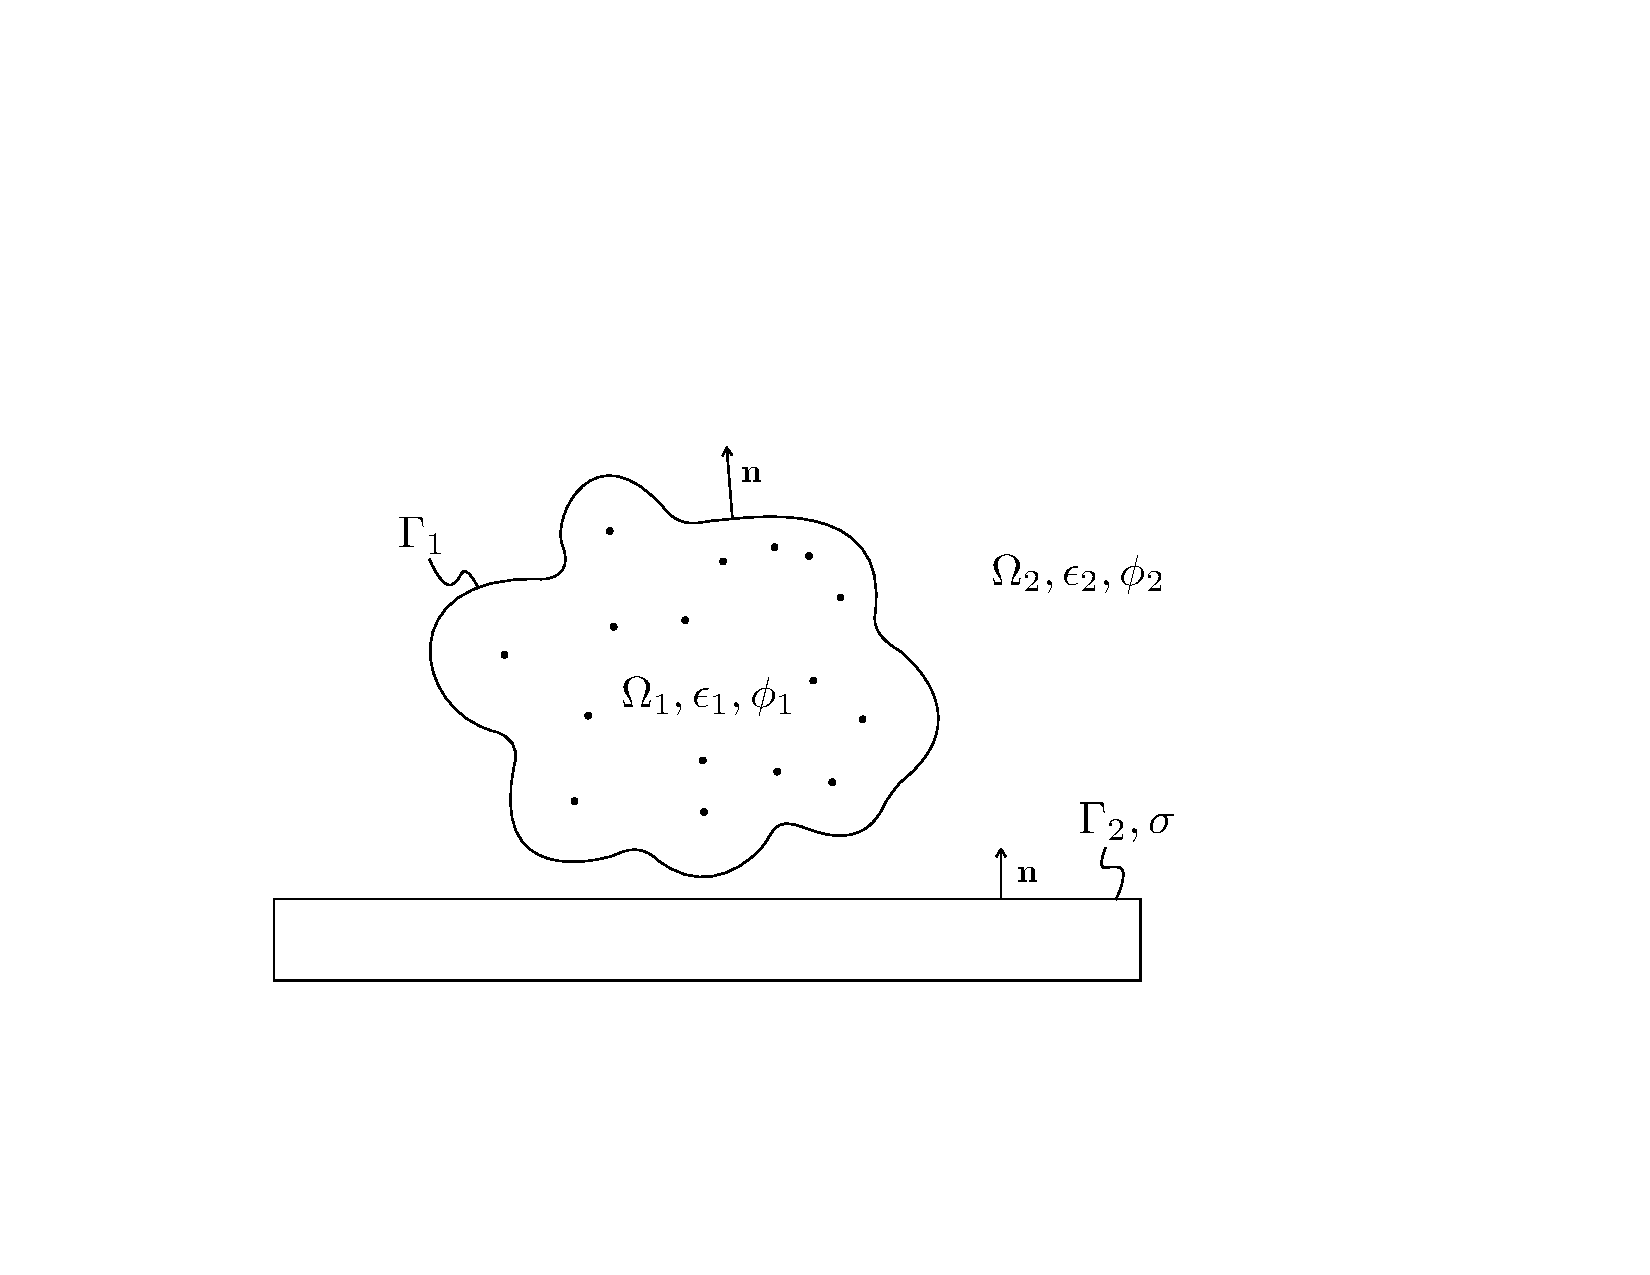
\includegraphics[width=0.45\textwidth]{Figure2.pdf} 
   \caption{Sketch of a molecule interacting with a surface: $\Omega_1$ is the protein, $\Omega_2$ the solvent region, $\Gamma_1$ is the  \ses and $\Gamma_2$ a surface with imposed charge.}
   \label{fig:molecule_surface}
\end{figure}
